\documentclass{article}
\usepackage{tikz}

\begin{document}

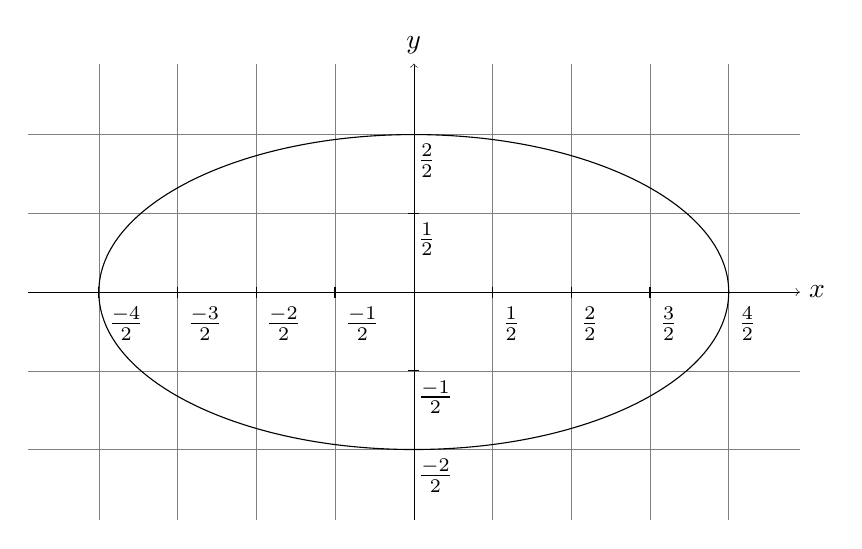
\begin{tikzpicture}

\draw[step=1cm,gray,very thin] (-4.9,-2.9) grid (4.9,2.9);
\draw[very thin,->] (-4.9,0) -- (4.9,0) node[anchor=west]  {$x$};
\draw[very thin,->] (0,-2.9) -- (0,2.9) node[anchor=south] {$y$};
\draw (0,0) ellipse (4cm and 2cm);
\foreach \x in {-4,-3,-2,-1,1,2,3,4}
\draw (\x cm,2pt) -- (\x cm,-2pt)
node[anchor=north west]{$\frac{\x}{2}$};
\foreach \y in {-2,-1,1,2}
\draw (2pt,\y cm) -- (-2pt,\y cm)
node[anchor=north west]{$\frac{\y}{2}$};
\end{tikzpicture}

\end{document}
